\chapter{Quantitative dynamics of histones in the human cell nucleus}
\label{ch:frap}

  %% FIXME this epigraph may not be acceptable...
  \epigraph{Agora desenmerda-te.}{Portuguese ``saying''}
  \noindent

  %% chapter concept: in this chapter goes the whole kill FRAP project. I started
  %% positive that this should work and so should the text. We start by studying
  %% the technique and list the assumptions it requires. We do one experiment and
  %% face some problems. Each problem has its own section that ends in a solution.
  %% When the solution was not done, we could offer one. The last one is the cause
  %% that this is not possible and has no solution. Conclusion lists all problems
  %% and their solutions again.

  \chapterprecis{
    To further the understanding of nucleosome structure and positioning
    in DNA, we aim to measure kinetic differences between wild type and
    mutant histones in live cells. Fluorescent Recovery After Photobleaching
    is a technique successfully used before to show the different kinetics and
    populations between histone types. Using the same approach with
    our most disrupting histone mutant, we test the limits of FRAP when
    faced with extremely slow exchange ratios.
  }

  \section{Introduction}

  \subsection{Histone contribution to nucleosome dynamics}

    The building block of eukaryotic chromatin structure is the nucleosome, comprising
    \SI{147}{\bp} of DNA wrapped around an octamer of two copies of core histones H2A,
    H2B, H3, and H4 \addref{Luger1997}. 
	Nucleosomes are arranged in a linear chain separated by DNA linkers, and
    can be further compacted into higher order chromatin structures. 
	The role of chromatin not only encompasses DNA compaction, 
	but also involves providing a dynamic complex to mediate access to genetic
    information by a capability to undergo reconfiguration of structure. \addref{Flaus?}

    Local reconfiguration of chromatin can be achieved 
	by changing nucleosome structure or altering its composition. 
	This can be performed through post-translational modifications or incorporation of histone variants, 
	causing nucleosomes to alter DNA sequence preferences or recruit other proteins.
	Alternatively, chaperones and ATP-dependent chromatin remodelling complexes
    act extrinsically in nucleosome position. 

	An important example of nucleosome remodelling is the SWI/SNF~complex
    whose deficiency causes growth defects in yeast.
	This complex was identified independnetly through screens for mating type SWIthching  \addref{?}
	or Sucrose Non Fermentation \addref{?}.

    A set of mutations have been uncovered that compensate for the loss of the SWI/SNF complex 
	that are collectively known as SIN mutations because they provide SWI/SNF INdependence  \addref{?}. 
	A subset of these are single amino-acid changes in core histones, 
	providing a direct link between SWI/SNF and chromatin and suggesting 
	that the histone mutation sites are involved in nucleosome dynamics and therefore
	of major importance in the nucleosome structure. This hypothesis has been tested \textit{in vitro} 
	where SIN mutant nucleosomes display higher thermal mobility \addref{Flaus EMBO} 
	and observed in crystal structures of the mutants \addref{Muthurajan 2004}.
	
	A complementary demostration of the effect of histone SIN mutants 
	in the more complex \textit{in vivo} chromatin environment would 
	validate the functional significance of these residues 
	and contribute to the understanding of conservation of histone sequences

	%% Leave out other mutants. Not everything we do is useful ...

  \subsection{FRAP}

    Fluorescence Recovery After Photobleaching (FRAP) is an optical technique
    that reveals the dynamics of fluorescently tagged molecules within live cells.
    The tagged molecules inside a small region are irreversibly photobleached by
    action of a high-power focused laser beam and the recovery rate of fluorescence
    is measured. The recovery rate is interpreted as unbleached molecules,
    which were outside of the region at the time of photobleaching, dissociating and
    diffusing into the bleached area, replacing the bleached molecules. It is assumed that the
    the fluorescence recovery reflects the protein natural movement.

    Its general idea can be described as chemical equilibrium:

    \begin{displaymath}
      F + S \overset{K_{on}}{\underset{K_{off}}{\rightleftharpoons}} FS
    \end{displaymath}

    where $F$ represents freely diffusing proteins, $S$ represents immobile vacant
    binding sites, and $FS$ the complex between the two, when the protein is bound
    to the binding site. This technique measures the value of \Kon{} and \Koff{},
    the association and dissociation constants, by observing how fast a
    small population of $F$ in the $FS$ complex, the ones that have been
    photobleached, is replaced.

    This technique has been extensively used to obtain qualitative and quantitative
    insight on the kinetic properties of proteins. Among these are also
    histone proteins, where FRAP was used to compare exchange ratios and
    soluble pools of different histones types and variants. These results
    show extremely slow recovery rates, with half-lives longer than 8~hours.

    %% FIXME we should probably be more descriptive of Kimura and Cook results

    Continuous development of FRAP has led to increasingly complex models
    that are both more precise and accurate than simple models based on
    inverse exponential decay.
    However, despite their sophistication, these models of recovery require
    certain important assumptions that are difficult to maintain for long
    experimental observation times:

    \begin{itemize}
      \item equilibrium is maintained throughout the entire experiment in
            order that both \Kon{} and \Koff{} remain constant, which requires
            that concentrations of both $F$ and $S$ remain constant;
      \item distribution of tagged molecule mimics the endogenous protein;
      \item the binding sites are part of a large, relatively immobile complex,
            at least on the time and length scale of the recovery.
    \end{itemize}

  \subsection{Objectives}

    We aim to develop a technique capable of measuring subtle kinetic
    alterations of the nucleosome in live cells which will allow us to study the
    structure--function relationship of the nucleosome.
    Since the histone SIN mutant H4~R45H has induced \textit{in vitro} the
    highest increase in nucleosome mobility, we will use it as positive
    control for testing FRAP for this purpose while at the same time
    validate \textit{in vivo} the previous results.

    The \textit{in vivo} results will lead to a more detailed model of the
    nucleosome, predicting effects of extra mutations that can be feed back
    to this technique for testing. A continuous cycle of this approach will
    lead to an increasingly refined model of the nucleosome.


  \section{Materials preparation}

%% This would need to be rewritten much more succinctly for a manuscript but is fine for thesis

  \subsection{Plasmid construction}

    Plasmids for the canonical histones H2B, H3, and H4,
    respectively pBOS--H2B--GFP \citep{KevinH2BGFP}, pBOS--H3--EYFP.MC--N1, and pBOS--H4--ECFP.M--N1,
    were provided by Prof. Kevin Sullivan from National University of Ireland,
    Galway (NUIG). DNA sequencing identified the H3 plasmid as the HIST1H3B gene, 
	encoding H3.1 from histone cluster 1; the H4 plasmid as either HIST1H4J or HIST1H4K; 
	and the H2B plasmid similar to HIST1H2BJ but with missense mutations D25G and V118I. 
	Plasmid pPAGFP--N1 and mCherry--\textalpha--tubulin were provided by Chelly van Vuuren 
	and the HeLa cDNA library was a kind gift of Nadine Quinn \citep{NadineThesis}. 
	Plasmid pMH3.2--614 including a mouse replication dependent histone~H3
    gene with upstream and downstream regulatory elements \citep{pMH3-plasmid},
    was provided by Prof. Kevin Sullivan.

    \paragraph{H2B--EGFP}
      The D25G and V118I mutations in pBOS--H2B--GFP were corrected by PCR mutagenesis 
	  using primers AFG114 and AFG115, and AFG112 and AFG113 respectively.
	  The resulting product is H2B--EGFP, equivalent to the HIST1H2BJ gene product fusion.

    \paragraph{H4--ECFP R45H}
      The R45H mutation was applied to the pBOS--H4--ECFP.M--N1 by
      PCR mutagenesis using the primers AFG124 and AFG125. The codon
      \texttt{CAC} was selected for the histidine amino acid due to its
      higher codon usage in the human genome\citep{codon_usage}.

    \paragraph{H2A--EGFP}
      Plasmid pBOS--H2B--GFP was digested with KpnI and BamHI 
	  and the band corresponding to the linearised vector without the H2B sequence 
	  was purified by gel extraction. The HIST1H2AB sequence was amplified 
	  from HeLa genomic DNA with primers AFG116 and AFG118 and ligated into the vector. 
	  This coding sequence is equivalent to the H2A used in the previous
      \textit{in vitro} studies to be compared \citep{flaus2004sin}.
      HIST1H2AE has the same gene product but a lower codon adaptation index 
	  and  more complex predicted 5' mRNA secondary structures.

    \paragraph{H2AX--EGFP and S139 mutants}
      Cloning of H2AX was similar to HIST1H2AB but used primers AFG130 and AFG131.
      Mutations to H2AX S139, an important site that is phosphorylated during
      DNA damage response, was performed at the same time of gene amplification 
	  since its location is close to the sequence 3' end. Primers AFG132, AFG133, and AFG134,
      were used with AFG130 to introduce mutations S139A, S139D, and S139E respectively.
	  The mutation to alanine blocks, while mutation to aspartic and glutamic acid 
	  mimic phosphorylation. This strategy introduced an accidental frameshift mutation 
	  near the stop codon which was fixed by PCR mutagenesis using primers AFG400
      and AFG401.

    \paragraph{H2A.Z--EGFP}
      The H2A.Z sequence was amplified from an HeLa cDNA library using primers AFG121 and AFG122 
	  due to the existence of introns in the H2AFZ gene. 
	  Purification of the amplicon and ligation to the linearised pBOS--EGFP vector
	  was identical to the preparation of the H2A--GFP plasmid.

    \paragraph{H4--EYFP}
      The plasmids pBOS--H3--EYFP.MC--N1 and pBOS--H4--ECFP.M--N1 were
      digested with the restriction enzymes BamHI and NotI. After agarose
      gel electrophoresis, the EYFP insert and pBOS--H4 vector were purified
      by gel extraction. The two DNA fragments were ligated to construct
      pBOS-H4-EYFP. The same strategy was used to construct the EYFP tagged
      H4~R45H mutant.

    \paragraph{H3--EYFP T45A and T45E}
      Mutations to H3 T45 were inserted into the pBOS--H3--EYFP.MC--N1 by
      PCR mutagenesis. The primers AFG151 and AFG152 were used for the
      T45E mutation, and AFG153 and AFG154 for T45A.

    \paragraph{H2B and H3 PAGFP}
      The PAGFP insert was prepared from pPAGFP--N1 by PCR using the
      primers AFG478 and AFG479, the amplicon purified by agarose gel
      extraction, digested with NotI and BamHI, and finally cleaned by
      PCR purification.
      Both pBOS--H2B--GFP and pBOS--H3--EYFP.MC--N1 plasmids were also
      digested with NotI and BamHI to excise their tags, and the vectors
      purified by agarose gel extraction. The insert was finally ligated
      into the two vectors for pBOS--H2B--PAGFP and pBOS--H3--PAGFP.
      This strategy introduces a Proline to Arginine mutation in the
      linker for the H2B plasmid.
      %% This mutation in the H2B linker (DPPVAT to DPRVAT) was on purpose.
      %% We could have easily avoid it but would cost us one extra primer
      %% and it shouldn't be making a difference.

    \paragraph{pMH2B--GFP and pMH3--EYFP}
      %% I'm actually not sure if Kevin gave me the pMH3.2--614 or the
      %% pCA-TAG plasmid. I did not have any plasmid map or sequence, only
      %% the very small Figure 5 of his paper PMID:9024683
      %% I couldn't even use any standard sequencing primer and by the time
      %% we cloned our genes there, we had already decided to kill the project
      %% so we never got to actually try these in human cells.
      Insertion of the H2B--GFP and H3--EYFP coding sequences into the
      pMH3.2--614 plasmid was performed by PCR amplification, bluent-end
      ligation of both vector and inserts due to the absence of restriction
      sites. pMH3.2--614 was amplified with primers AFG417 and AGF418 which
      create a linear sequence that only ignore the H3.2 coding sequence.
      The H2B--GFP coding sequence was generated with primers AFG419 and AFG420.
      Primers for the insert were phosphorylated by T4~PNK prior to the PCR
      since T4~PNK is more efficient on single stranded DNA. pM vector and
      H2B--GFP insert were purified by agarose gel extraction and ligated.
      Strategy for H3--EYFP was equivalent but using primers AFG424 and AFG420.

  \subsection{Cell lines}

    Transfection was always performed by lipofection~(\Sref{methods:lipofection}),
    both for transient and stable cell lines. For creation of stable cell lines, 
	cells were trypsinized and split 1:20 on \SI{10}{\cm} dishes 24~hours after transfection.
    After another 24 hours, Blasticidin-S was added to the medium for
    a final concentration of \SI{3}{\ug\per\ml} as found by performing a
    Blasticidin-S kill-curve (\Sref{sec:methods:kill-curve}).
    Cell growth was followed and medium replaced when appropriate.
    As cell colonies started to be visible by the naked eye, approximately
    3~weeks after plating, these were screened by fluorescence microscopy.
    Positive colonies were aspirated and moved into 24-well plates with
    \SI{1}{\ml} disposable pipette tips, and the thinnest extremity removed.

    \begin{figure}
      \centering
      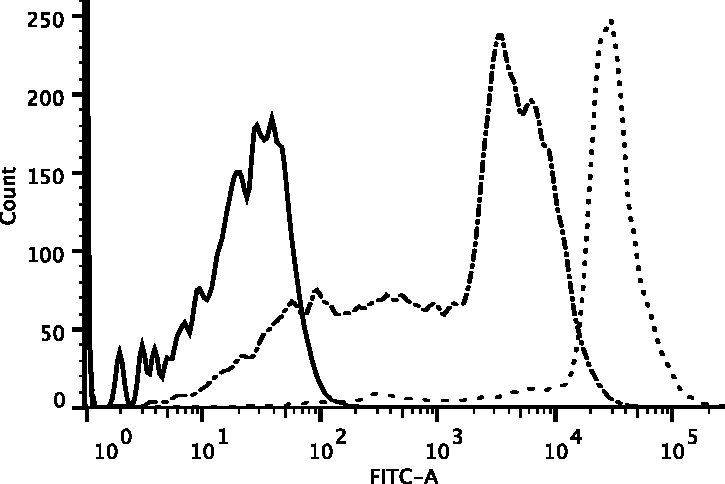
\includegraphics[width=\textwidth]{facs-stable-cell-lines.pdf}
      \captionIntro{FACS sorting of mixed populations}
        {
          The multiple populations with differing intensity values were
          sorted by FACS. The full line represents the intensity profile
          of HeLa wild type cells; the dash-dot line, a mixed population
          of HeLa cells expressing H2B--EGFP; and the dotted line, the
          sorted population.
        }
      \label{fig:methods:facs}
    \end{figure}

    Populations with mixed levels of fluorescent intensity were frequently
    obtained while preparing stable cell lines. In such cases, cells with
    similar intensity of their corresponding fluorophore were FACS
    sorted (\fref{fig:methods:facs}).

    The following stable lines were prepared:

    \begin{itemize}
      \item HeLa H2B--EGFP
      \item HeLa H2B--EGFP D25G V118I
      \item HeLa H3--EYFP
      \item HeLa H3--EYFP T45A
      \item HeLa H3--EYFP T45E
      \item HeLa H4--EYFP
      \item HeLa H4--EYFP R45H
    \end{itemize}

  \subsection{Microscopy}

    Both stable and transiently cell lines were used in imaging as described. 
	Transfection was performed approximately 48~hours before imaging for transfected cells.
	%% Can you be a bit more exact than approximately? Give a time range?

    Confocal microscopy was performed with a Zeiss LSM510 Meta microscope
    using glass bottom LabTek II chambers. Wide-field fluorescence microscopy
    was performed with an Applied Precision DeltaVision Core system
    using \SI{35}{\mm} glass bottom MatTek dishes.

    In both cases, imaging was performed within an acrylic environmental
    chamber that fully enclosed the stage plate and microscope objectives.
    Temperature and CO$_2$ levels were maintained via separate units connected
    to the environmental chamber.

  \subsection{Computational analysis}

    Software used for image analysis and visualization was described in
    \Sref{sec:methods:software}. Original source code written in \textsc{Matlab} for a previously
    reported circle FRAP model \citep{mueller2008evidence} was kindly offered
    to us under the GNU General Public License (GPL) version~3 by the
    original authors. A port of this code for the GNU Octave language was
    prepared and made available under the same license.


  \section{The required time frame}
  
  While the FRAP model we are using works best when complete recovery is observed, it could be
  possible to observe some change on a fast exchanging population at the start of the recovery.
  
  Since the histone mutant which had shown the highest \textit{in vitro} effect on nucleosome
  was H4 R45H, we used it as starting point for testing this. We performed a 90 seconds FRAP
  experiment with it, H3 T45A, and H4 WT but at were unable to find a noticeable\todo{be specific}{} difference
  (\fref{fig:90-sec-frap}).
  
  \begin{figure}
    \centering
    \missingfigure{plots comparing H3 T45A and H4 and H4 R45H \Kon and \Koff}
    \captionIntro{\Kon and \Koff values estimated from 90 seconds FRAP experiment.}
                 {}
    \label{fig:90-sec-frap}
  \end{figure}
  
  We then tried to simulate how a recovery curve for a single population of proteins with
  residence times of 9 and 7 hours would look like (\fref{fig:simulated-frap}). We assumed
  that these were reasonable values given Kimura and Cook paper. This had shown us that indeed
  the initial 90 seconds would not be enough to measure a difference on the microscope.
  
  \begin{figure}
    \centering
    \missingfigure{comparison of recovery of 2 proteins with residence time of 9 and 7 hours}
    \captionIntro{Simulated recovery curves of proteins with long residence times.}
                 {}
    \label{fig:simulated-frap}
  \end{figure}
  
  Considering the typical fluorescence intensity we observed on our cells (around\todo{!!be accurate}{} 40\todo{unit?}), and the simulated curve,
  it would require at least 1 hour of recovery until the difference in intensity between the two was of 1, so
  we could see with our microscope camera. Of course, this is the minimum, and considering the noise, we need
  much much more. At least 4 hours would be required to obtain data to validate any difference, and even then,
  more should have been used.

  \todo[inline]{\textbf{Andrew notes:}
                
                Add references. Significant. Explain ref. Exact values. Be accurate}

\section{Cell movement}

  While most FRAP experiments are done on a short time scale where the cell movement
  is not noticeable, the low recovery rates of histones requires collection of images
  over several hours. \addref[Kimura and Cook] reported that the recover was not
  complete, even after 8h for H2B--EGFP, the time frame we used for our initial experiments.
  On time series experiments with of such long
  times, cell movement becomes a issue (\fref{fig:cell-movement}) thus requiring tracking
  of the cell nuclei\todo{expand explanation}. This is assuming that we want to automate the analysis of course.
  Would not be a problem if we had trained monkeys drawing regions by hand.
  
  \begin{figure}
    \centering
    \missingfigure{HeLa cells moving around}
    \captionIntro{Long time series of HeLa cells expressing H2B--EGFP.}
                 {Cells were transfected with pBOS--H2B-EGFP and imaged for 8
                  hours, with intervals of 20 minutes.}
    \label{fig:cell-movement}
  \end{figure}
  
  We tried different approaches to solve this issue.
  
  \subsection{Higher cell density}
  
    Our first attempt to limit the movement of the cells was to perform the experiment with
    cells at higher cell density.  Contact between cells is a factor that usually inhibits
    their movement, a characteristics named ``contact inhibition''\addref[Density Dependent Inhibition of Cell Growth in Culture].
    
    However, HeLa cells did not seem to respect this, and kept moving around, even crawling
    over each other in occasions. This probably comes from the fact that HeLa cells are fucked
    up cancer cells with little respect for anything other than I want to multiply.
    
    We did notice a decrease on movement, probably due to the fact that the cells did have less
    space to move around, the dish was more crowded. Still, this was not enough\todo{expand}.

  \subsection{Primary cell lines}
  \label{sec:frap-movement-horse}
  
    The issue with HeLa cells is that they are cancer cell lines where all the checks that typical
    healthy cells are ignored. As such, we attempted the same approach with a primary cell line\todo{explain}.
    
    We used a horse fibroblast cell line as these are reported to stop growth once they have reached
    confluence. They are reported to create a tissue layer of healthy cells and not move. Their main
    disadvantage, aside from more difficult handling and limited passage number, is the much greater
    difficulty of transfection, with a much lower \todo{resultag. be specific of typical range)} transfection efficiency. Also, these cells are not
    so standard which would make taking comparisons from other studies less conclusive.
    
    We made an initial check that the horse cells would indeed stay healthy after reaching confluence.
    We let them reach confluence on a dish and left them alone\todo{alone?} for 2 weeks, only changing the growth
    media every 3 days. After this time the cells had formed a tissue layer and looked healthy (\fref{fig:healthy-horse}).
    \todo{healthy? be scientific. Criteria?}
    
    \begin{figure}
      \centering
      \missingfigure{Horse nucleus cells looking healthy after 2 weeks}
      %% TODO we need to redo this experiment, this time with glass bottom for imaging after.
      %%      Problem may be that when doing the staining, some cells will be washed away and
      %%      will look fake. We can take an image before the washing to explain that.
      %%      something better than just DAPI to show that the cells are actually healthy?
      %%
      %%      Just some viability test using trypan blue, and compare against the cells kept growing
      \captionIntro{Effect of contact inhibition on primary horse cell line.}
                   {The cells were left on the dish for 2 weeks after reaching confluence. The
                    image on the left is the bright field image before staining and fixation.
                    The cells on the right are the DAPI staining for better view. The missing
                    areas is due to the washing steps involved with the staining.}
      \label{fig:healthy-horse}
    \end{figure}
    
    Happy\todo{happy?} with this, we transfected the cells with H2B--EGFP and assess the reduction in movement.
    The transfection efficiency was much lower than when using HeLa as expected (this was checked 2 days
    after transfection). We imaged the cells over 8 hours but cells moved anyway (\fref{fig:horse-moving}).
    \todo{discuss level of movement}
    
    \begin{figure}
      \centering
      \missingfigure{Time series of horse cells expressing H2B--EGFP moving after 8 hours}
      \captionIntro{Movement of primary horse fibroblast despite contact inhibition.}
                   {The cells were transfected with H2B--EGFPat high cell density and
                    imaged over 6 hours. They still moved, and even spiralled.}
      \label{fig:horse-moving}
    \end{figure}

    %% We never tried serum starvation


  \subsection{CropReg}
  
    To solve this problem, we developed a computer program named CropReg\footnote{The name CropReg
    comes from the program flow, a loop between image cropping and image registration.}. This
    program implements template matching \todo{image registration vs template matching} by
    finding the maximum in the normalized cross-correlation matrix of a
    box enclosing the nucleus of interest (the template) and the following frame (\fref{fig:normxcorr2}). The
    coordinates of the maximum correspond to the coordinates where the template matches the ``best''\todo{criteria?}{} on the
    image. This new coordinates are then used to create a new template which is used to search for the nucleus
    on the following time point.
    
    For performance reasons, rather than using the whole image of the following time point, the area surrounding
    the one on the previous time is used.
    
    \begin{figure}
      \centering
      \missingfigure{Explaining normalized cross correlation. 3 images. First is $f_n$ with a box
                     around the cell that will be used as template $t$. Second image is $f_n$ with the
                     cells moved a bit. Third image is the normalized xcorr2 output as a 3D landscape
                     with an arrow pointing to the max peak.}
      \captionIntro{Using normalized cross-correlation for tracking of cell nucleus.}
                   {The left image, $f_n$
                    The box around the nucleus of interest, $t$, will be the template for the cross-correlation.
                    The center image, $f_{n+1}$, is the image on the time point after $f_n$. The right image is
                    the surface mesh plot of the normalized $(t \star f_{n+1})$.}
      \label{fig:normxcorr2}
    \end{figure}
    
    %% TODO since there's more than one way to actually do the normalization, it might be
    %% a good idea to writedown the actual math formula
    
    %% FIXME we could use the listings package which will look nicer and let us have the actual
    %%      code on a separate file to not break the indentation
    
    \begin{verbatim}
## a is the image
## b is template
c = conv2 (a, conj (b (rows(b):-1:1, columns(b):-1:1))); 
a = conv2 (a.^2, ones (size (b)));
b = sumsq (b(:));
c(:,:) = c(:,:) ./ sqrt (a(:,:) * b);
\end{verbatim}
    
    \todo[inline]{ materials and methods? Or appendix? Code in the middle of chapter not typical}
    
    This is the code for the normalized cross-correlation which is at the core of CropReg. Rather than having
    it for ourselves only, it was implemented as a new option for the xcorr2 function and released under GPLv3+ with
    the Octave Forge signal package version 1.2.0. The function normxcorr2 was released as a wrapper for
    this option, with the image package version 2.0.0.
    
    This algorithm is able to track cell nucleus efficiently\todo{criteria}, as long as cell nuclei of different cell do not
    overlap\todo{And when they touch... some morphology to count number of nuclei and if two, check with using the
    center of the template.}(\fref{fig:cropreg}).
    
    \begin{figure}
      \centering
      \missingfigure{}
      \captionIntro{CropReg in action.}
                   {This will actually be 3 subfigures. First is finding the nucleus of intereste by image subtraction.
                    Second is just CropReg. Thirs is accounting for image rotation.}
      \label{fig:cropreg}
    \end{figure}

    Two problems are left to solve: nucleus rotation (rotational movement of the nucleus on the
    Z axis) and finding the template for the first image. The first
    was solved by using the StackReg plugin for ImageJ\todo{we should write it in Octave and add it to cropreg}
    \addref[we need to reference it if we do use it]. The second was using by subtracting the post bleach to the
    pre-bleach image, threshold the image, remove noise and use it as marker to select the right nucleus\todo{demonstrate}.

\section{Cell cycle --- System equilibrium}
\label{sec:frap-equilibrium}

%% There's no chemical equilibrium in S phase <-- Kevin sullivan

  Another consequence of long time experiments is that the experiment will start to span
  multiple cell cycle phases. We were using HeLa cells which have an average doubling time of 24h.
  Since the experiment are at least eight hours long, and the experiment can not cross mitosis,
  it is problematic to perform it so that it does not cover part of S~phase (\fref{fig:cell-cycle-watch}),
  where\todo{there's problems}.
  
%  \begin{wrapfigure}{o}{0.5\textwidth}
  \begin{figure}
    \centering
    \missingfigure{a small figure, probably should be a float with wrapping}
    \captionIntro{Cell cycle watch.}
                 {Too short cell cycle and too long experiment.}
    \label{fig:cell-cycle-watch}
  \end{figure}
%  \end{wrapfigure}
  
  The histone expression profile is atypical in that it is mainly expressed during S~phase, with
  a 35-fold up-regulation\addref. This is a consequence of the requirement for large amounts of
  canonical histones during S~phase to package the newly duplicated genome\todo{reference section
  on histone catalogue or introduction where I talk about this}.
  
  This breaks the assumptions of the FRAP model that the system remains in equilibrium. This can be
  expressed as a simple chemical reaction:
    
  \begin{displaymath}
    F + S \overset{K_{on}}{\underset{K_{off}}{\rightleftharpoons}} C
  \end{displaymath}
  
  where $F$ represents the freely diffusing proteins, $S$ represents the vacant binding sites, and
  $C$ the $FC$ complex when the protein is bound to the binding site while we try to measure the
  values of \Kon and \Koff, the association and dissociation constants.
  
  The assumption is that this equilibrium has been reached when we start the FRAP experiment and
  continues so that \Kon and \Koff remain constant throughout the experiment. This does
  not hold for S~phase where there is an increase of $F$ and $S$ because the new histones being expressed
  and the new duplicated genome. Adding more reactants to a system in equilibrium will change the equilibrium
  constants so the fluorescence recovery will not be interpretable.
  
  \subsection{Contact inhibition}
  \label{sec:frap-cell-cycle-horse}
    
    As effect of contact inhibition is that cells showing this behaviour should stop cell
    growth when reaching confluence. Once reaching a certain state, the cells should move from
    the G$_1$ into the G$_0$ phase where they are arrested until the inhibition stops.
    
    Similar to the approach we took for the cell movement, we used a primary horse fibroblast
    cell line that showed contact inhibition.
    
    \begin{figure}
      \centering
      \missingfigure{FACS of horse cells after 2 weeks on dish and full}
      \captionIntro{FACS of primary cells showing contact inhibition.}
                   {Control is the horses that have been kept growing for the 2 weeks,
                    being split every 3 days, while horse cells were left on dish for
                    2 weeks, changing media only every 3 days.}
      \label{fig:horse-facs}
    \end{figure}
    
    This approach showed success \todo{detail} but the cells showed a much lower transfection efficiency\todo{detail}. This
    would have been a good approach if the use of this cells had also solved the problem of cell
    movement. Therefore, picking cells was better.

  \subsection{Selection of G$_1$ cells}
  
    To avoid changing cell cycle, and the use of drugs for blocking cell growth, during a
    continuous time interval of eight hours, the only cell cycle phase that lasts sufficiently
    long is the G$_1$ phase (\fref{fig:cell-cycle-watch}). So the ideal cells to perform this
    experiment are cells that are at the beginning of G$_1$ phase.
    
    To be certain of the cell cycle phase at the start of the experiment, we began by selecting
    cells that were entering mitosis. We imaged these cells for 4 hours and used the daughter cells
    for the FRAP experiments (\fref{fig:picking-cells}).
    
    \begin{figure}
      \centering
      \missingfigure{Hela cells splitting}
      \captionIntro{Picking cells at early G$_1$.}
                   {We imaged cells that were entering mitosis and picked their
                    daughter cells for the FRAP experiments. Because HeLa cells lift
                    away from the dish during mitosis, opening the
                    pinhole and set the Z-center in between the cell dividing plane
                    and dish bottom was necessary. Ends up nothing being properly in focus but we
                    can track things fine. Of course, some cells still floated away.}
      %% TODO explicit parameters
      \label{fig:picking-cells}
    \end{figure}
    
    Directly after mitosis, there is an interval of a couple of \todo{approximately how many}
    hours for chromatin to decondense and reorganize\addref. So cells are\todo{??uasmittle?? directly}
    Kimura has recently found fancy dynamics for DNA binding proteins \addref[some ring like shaped protein
    from what Tim was working on] on the first 3 hours of G$_1$\addref.
    
    \todo[inline]{look for papers from Andrew Belmont. Search finite time potential 'spatial disequilibrium'.}

  \subsection{Drugs}
  
    Drugs should be avoided. Different drugs had different effects on Kimura and Cook paper.

    \begin{figure}
      \centering
      \missingfigure{tracking stable mRFP--PCNA cell lines for a long time after picking them after mitosis}
      \captionIntro{Measuring length of G1 phase}
                   {Control is the horses that have been kept growing for the 2 weeks,
                    being split every 3 days, while horse cells were left on dish for
                    2 weeks, changing media only every 3 days.}
    \end{figure}

  \subsection{Alternative cell lines}
  
    An alternative would be to pick cell lines with longer cell cycles (\tref{tab:alternative-cells}).
    
    \begin{table}
      \missingfigure{actually a tabular environment listing some alternative cell lines}
      \caption{Table of cell lines with cell cycles longer than HeLa.}
      \label{tab:alternative-cells}
    \end{table}


\section{Tagged protein distribution}
  \todo[inline]{keep flow of story}
  An obvious assumption of the model is that the distribution of the tagged protein mimics
  the distribution of the endogenous protein. It was proposed by \addref[Kimura and Cook] that
  this does not hold, which explained the abnormal distribution of H2B--GFP on the cell nuclei.

  %% we could also write this by first mentioning the two types of regulation and explaining them
  %% and them showing how the pBOS plasmid fails with both
  The non-linear expression of the histone proteins previously mentioned (\Sref{sec:frap-equilibrium}),
  is controlled at two stages. On a first level, there is an increase of transcription during S~phase
  but this only accounts for part of the the increase. At a second level, the stability of the histone
  transcripts also increases at S~phase \todo{reference to the introduction where I mention this}.
  
  Unlike all other eukaryotic genes, histone transcripts lack a poly(A) tail, encoding instead a
  stem--loop and a purine-rich Histone Downstream Element (HDE) downstream of the stop codon.
  These two structures, which are not part of the coding sequence, are involved in the
  mRNA stabilization and further responsible for the expression profile of histones.
  
  The pBOS--H2B--EGFP plasmid does not respect any of these control elements. The promoter of the EF-1\textalpha{} gene, used in the
  pBOS plasmid is unregulated leading to constitutive expression of the tagged protein. This will guarantee different
  distributions of tagged versus endogenous proteins on the free pool over time. Since the duplication
  of genome is not equal, there is more heterochromatin duplicated at the end of S~phase, while
  euchromatin is duplicated at the start, so the distribution of the tagged histones will be skewed so that there's
  more of it on the euchromatin, when the proportion of tagged histones is
  higher (\ref{fig:mess-histone-expression}).
  
  \begin{figure}
    \centering
    \missingfigure{a scheme like the one in Himura and Cook paper.}
    \captionIntro{Distribution of tagged histones on free pool over time}
                 {Profile of free pool size on typical case vs our experiment. Use
                  different colors under the curve to show the different proportions.
                  Separate plot for the actual expression}.
    \label{fig:mess-histone-expression}
  \end{figure}
  
  Of course, no one actually tested this, can be quite tricky to this with proper controls\todo{scientific writing}. And we also
  don't know that if in the case of the overexpression, the cell would at translation or protein degradation
  level. There's chaperones specialized in degrading histones. Kevin seems to believe so. This would
  also explain Kimura and Cook results with the weird distribution if the difference on dynamics
  between H2B and H3 also holds\todo{good point. Be more analytical and discuss}.
  
  I actually tried to perform subcellular fractionation with a protocol from Ronan which is on the wiki.
  The signal of the tagged histone, in relation to the endogenous, was quite high. But the western
  looked like crap, many non-specific bands. Couldn't see with the H3 antibody but something went
  wrong with that lane (it was the one that turned yellow during the boiling of the sample). Now that
  I have the samples, I could try an H3 antibody for a H3 PTM which didn't work before.
  
  \todo[inline]{need to show data or explain problem or not mention! Jenn could help? "preliminary expt (data not show)"}
  
  While getting the promoter right is a bit tricker, cloning the stem loop and removing the poly-A tail
  is much more straightforward, and is a care that should be taken when doing this. It has been reported
  that the downstream elements have a bigger impact on the expression than the promoter. Luckily, this
  is also the part that should be easier to fix with cloning.
  
  We used a plasmids that Kevin used a long time ago, where he cloned an H3 gene from mouse on its
  entirety and only added a tag to the H3 gene, keeping the rest intact\addref[Kevin's paper
  with the plasmid used in mouse].
  
%%  We started to work on it but did not had any plasmid map,
%%  or sequence, other than a very small picture from the paper where he published with very
%%  bad quality. We couldn't even use any standard sequencing primer. We ended up not doing
%%  any work on it since by the time we got it, we were already noticing all
%%  the other issues with the project.

  %% on the case of proteins with special control of expression, may make sense to look into it.
  %% Specially if the proteins will have very slow exchange rates this may affect its distribution.
  
  %% Solution may be to clone to whole gene. In some cell lines (DT40) it's very easy to knock in
  %% a gene and tag the endogenous. When zinc-finger technology becomes more accessible it may
  %% become possible to use it on more common human models.


\section{Chromatin movement}
  
  During some FRAP experiments, we observed major changes in the shape of the bleached area due to
  chromatin movement (\fref{fig:frap-chromatin-movement}). This is difficult to assess because of the
  non homogeneous nature of chromatin and the whole nucleus being stained green.
  \todo[inline]{give descriptive idea of nature of changes}
  
  \begin{figure}
    \centering
    \missingfigure{original H2B-EGFP FRAP experiment with bleached hole acting like a contortionist}
    \captionIntro{H2B--EGFP FRAP experiment showing chromatin movement.}
                 {mention time interval and whatever}
    \label{fig:frap-chromatin-movement}
  \end{figure}
  
  The assumption that the binding sites, in this case chromatin, remain immobile through the FRAP experiment is
  required in order to interpret the recovery of fluorescence as free unbleached molecules moving
  into the bleached area and associating with the binding sites, an effect of the association rates \Kon and
  \Koff. If chromatin itself reshapes and moves unbleached molecules from outside into the bleached area, then
  the recovery is also a function of the binding sites movement. Without a model for this movement, it is not
  possible to separate the two functions, and obtain the association rates.
  
  To correct for this movement, it would be necessary to visualize it independently. The standard method when doing such long
  FRAP experiments is to use histones for control, where they are usually perceived as being immobile. We are
  at the limit, on the time scale of the experiments we need to do, nothing in the chromatin can be assumed
  to be immobile. A possibility would be to stain the actual DNA but the molecules would still exchange faster
  than the histones.
  
  To have a better look\todo{better look?} at this, we performed inverse FRAP (iFRAP), where instead of bleaching a small region
  and measure the fluorescence recovery, the protein is tagged with PA--GFP, a small region is
  activated, and its fluorescence decay is measured. Because PA--GFP is invisible before the photoactivation,
  we co-transfected cells with mCherry--\textalpha--tubulin. When performing co-transfection, it's more likely
  that cells have incorporated both plasmids\todo{prove this where?}, so expression of
  mCherry--\textalpha--tubulin is a good indication that it is also expressing H2B--PA--GFP. The use of
  \textalpha--tubulin is also a good indicator of the nucleus boundaries which is a visual aid for this
  experiment (\fref{fig:ifrap-chromatin-movement}).
  
  \begin{figure}
    \centering
    \missingfigure{inverse FRAP experiment showing chromatin movement}
    \captionIntro{inverse FRAP experiment showing chromatin movement.}
                 {mention time interval and whatever. We have co-transfected cells with \textalpha--tubulin
                  tagged with mCherry to find cells that had been transfected and to visualize the borders
                  of the nucleus}
    \label{fig:ifrap-chromatin-movement}
  \end{figure}
  
  With this set up, we were able to notice that the movement of chromatin was indeed more frequent and of
  bigger \todo{more and bigger? quantitative measurement?}
  impact that what the ``normal'' FRAP experiments originally suggested. We also note that even with
  iFRAP, it is not possible to be sure whether chromatin movement has occurred. If intensity in the activated
  region drops by 4 for example, and we can't see those 4 in another location (or locations) of the nucleus,
  it can still be
  that the chromatin that holds those 4 are spread over a larger region which is perfectly reasonable if the
  chromatin is movement and it is likely to be below the sensitivity of the camera.
  
  And the low intensity and greater sensitivity to bleaching of PA--GFP when compared to EGFP, just makes this
  even worse.
  
  We though that this problem would be related with cell movement and could be
  corrected by using a cell line with contact inhibition but this did not happen (see \Sref{sec:frap-cell-cycle-horse} and
  \Sref{sec:frap-movement-horse}).

  \todo[inline]{chromatin is not homogeneous. Different parts of the chromatin should have
                different recoveries. Where can I mention this?}



  \section{Discussion}

  Performing FRAP of histones requires an extension of the experiment over
  its typical length. \cite{KimuraCook}
  reported that the recovery was not complete, even after 8~hours.
  We aimed at compare kinetic constants of wild type histones against
  specific mutants, and used a previously reported model for circle FRAP
  which had already been validated against other fluorescent techniques,
  and reported to account for multiple errors in a typical FRAP modelling.

  However, simply collecting valid recovery data for such a long time
  period is an issue on its own.

  \subsection{Cell movement}

    The first problem to expect when performing such experiment over
    long times is cell movement. This is a natural occurrence and cells
    where movement is absent are likely to be dead. But as the nuclei
    movement is mostly translational and rotational around the $z$ axis,
    a single spot can still be tracked in a single focal plane.

    \label{sec:kill-frap:discuss-contact-inhibition}

    We attempted to eliminate cell motion by inducing contact inhibition,
    a feature of normal cells to control cellular growth. As cells reach
    higher densities, they move into the \G0{}~phase of the cell cycle,
    entering a quiescent state. In tissue culture,
    this translates to a stop in proliferation, and formation of a monolayer
    of healthy cells in the flask. This requires the use of primary
    cell lines since these have not lost this feature yet.

    This is a very attractive strategy for reducing motion due to the
    fact that this is a natural occurring mechanism. Nonetheless,
    other factors must be taken into consideration.
    Increased difficult on cell handling, and reduced
    transfection efficiency are only labour related, but it also means
    that stable cell line cannot be used. Most importantly, immortalized
    cell lines such as HeLa are standard in cell biology which makes
    comparisons to other studies much more conclusive.

    However, while we did observe a monolayer of healthy cells develop,
    and maintained stable over 2 weeks, observation of individual transfected
    cells still showed movement. In addition, the nature of the movement
    had changed and instead of the simple translational movement observed
    in the HeLa cells, all nuclei displayed an helix-like movement on the
    direction of the movement (\fref{fig:kill-frap:confluent-horse}).

    %% Meth! Not even once.
    The possibility of using drugs to reduce motion was also briefly
    considered. Previous FRAP of histones was performed using
    multiple inhibitors of protein synthesis, which reported different
    histone kinetics for the same histones \citep{KimuraCook}. Their
    conclusion was that the results were ``difficult to interpret''.

    Ultimately, we solved this problem by writing our own program
    for cell tracking by normalized cross-correlation template matching, a
    well-known technique. Not only was this technique sufficient for our
    case, it also avoided the usage of any drugs that could affect the
    conclusions and add another variable.


  \subsection{System equilibrium}

    The basis behind a FRAP experiment is a chemical equilibrium on
    formation of a complex between the freely diffusing proteins and
    vacant binding sites, and for the equilibrium to be maintained,
    concentrations of both reactants must remain constant.
    When the system is the intra cellular environment, achieving
    true chemical equilibrium is inconceivable but for the purpose
    of a FRAP experiment, certain efforts can be taken to reach a
    compromise.

    In our specific case of FRAP for histone
    dynamics in chromatin, the equilibrium is between
    a soluble pool of histone proteins, and formation of a nucleosome
    bound to the DNA. This translates in a requirement to maintain the
    amount of proteins and DNA constant. If FRAP was performed in the
    time-scale of seconds or even minutes, 

    \subsubsection{DNA replication}

      %% Interesting: the paper "A search for differential polypeptide synthesis
      %% throughout the cell cycle of hela cells", on Journal Cell Biology 1980,
      %% vol 84 795-802 by Rodrigo Bravo and Julio E. Celis, says about HeLa
      %% cell cycle on page 796 that "average duration of G1, was 11.7 h; S was
      %% 8.8 h; and G2 and M was 4 h. The division time was 24.5 h." However,
      %% the technique they refer mention much shorted times.
      %% They reference "Growth and nucleic acid synthesis in synchronously
      %% dividing populations of HeLa cells", on Experimental Cell Research
      %% 1963, vol 30 344-362 by T. Terasima and L.J. Tolmach which on Table III
      %% in page 354 have a median doubling time of 21h (which is actually quite
      %% shorter than the typically reported 24h for HeLa under optimal
      %% conditions), and 8.5h for G1, 9.5h for S, 2.3 for G2, and 0.7h for M.
      %% So HeLa cells from the 60s are different from the cells of nowadays?

      \begin{figure}
        \centering
        %% based on original code from Robert Vollmert
        %% http://www.texample.net/tikz/examples/pie-chart/
        \newcommand{\slice}[4]{
          \pgfmathparse{0.5*#1+0.5*#2}
          \let\midangle\pgfmathresult

          % slice
          \draw[thick,fill=black!10] (0,0) -- (#1:1) arc (#1:#2:1) -- cycle;

          % outer label
          \node[label=\midangle:#4] at (\midangle:1) {};

          % inner label
          \pgfmathparse{min((#2-#1-10)/110*(-0.3),0)}
          \let\temp\pgfmathresult
          \pgfmathparse{max(\temp,-0.5) + 0.8}
          \let\innerpos\pgfmathresult
          \node at (\midangle:\innerpos) {#3};
        }
        \begin{tikzpicture}[scale=3]
          \newcounter{a}
          \newcounter{b}
          %% Total cell cycle is 24.5 hours, G1 is 11.7h, S is 8.8h,
          %% G2 is 3h, M is 1h. The problem is that the counters can't handle
          %% decimal places so we have a variable with the actual time for
          %% the text, and another one times 10 to calculate the angle.
          \foreach \p/\t/\l in {117/11.7/\G1, 9/0.9/M,
                                31/3.1/\G2, 88/8.8/S}
            {
              \setcounter{a}{\value{b}}
              \addtocounter{b}{\p}
              \slice{36*\thea/24.5} % we multiply by 36 instead of 360 because
                    {36*\theb/24.5} % the time is already times 10
                    {\l}{\t{} hours}
            }
        \end{tikzpicture}
        \captionIntro{HeLa cell cycle phases and choice of timing}
          {
            Under optimal growth conditions, the HeLa cell has a median
            doubling time of approximately 24.5~hours, with \G1~and
            S~phases alone having a length of 11.7 and 8.8 hours each \citep{HeLaCellCycle}.
            Since the FRAP experiment must avoid the S phase and last for
            at least 8~hours, the only possibility while using cells in normal
            growth conditions is to start the experiment in the early \G1~phase.
          }
        \label{fig:kill-frap:cell-cycle}
      \end{figure}

      %% How we got to 3.1 hours for G2 phase: in 1980, they reported 4h
      %% for G2 and M phases together. In 1963 they specified 2.3 and 0.7
      %% for each, so the total increased by 1/3 (from 3 to 4 hours).
      %% I'm assuming 2.3 + 2.3*1/3

      DNA replication happens during the S~phase which breaks the equilibrium.
      In addition, the entire replication machinery will move through the DNA
      strands, displacing nucleosomes. This limits the experiment from the
      interphase to either \G1{} or \G2{} phases. However, considering
      the HeLa cell cycle has an average \G2{} phase of 3~hours, and even
      \G1{} is 11.7~hours long \citep{HeLaCellCycle}, the FRAP experiment
      becomes limited to a start on early \G1{} (\fref{fig:kill-frap:cell-cycle}).

      %% papers from Andrew Belmont. Search finite time potential 'spatial disequilibrium'

      %% When I was at Jim McNally's lab, Timothy Stasevich was leaving to
      %% work on Hiroshi Kimura's lab and heard that he had found some
      %% fancy dynamics for DNA binding proteins on the early 3 hours of G1.
      %% It was not published back then, and I couldn't find it.
      In addition, post-mitotic chromosomes take some time to rebuild the
      interphase nuclear architecture during early \G1{}. After decondensation,
      chromosome territories move within the nuclei to similar neighbourhoods
      as their mother nucleus, a process that has been estimated to
      take approximately 2 hours
      \citep{visualizationG1chromosomes,earlyg1position,RelativeChromosomePosition}.
      This further limits the timing to start a FRAP experiment to a very
      small window.

      We solved this problem in a rather ingenious method, minimizing
      intervention on the cell normal growth. We tracked cells manually during
      mitosis where visual identification of the cell cycle is possible,
      therefore limiting the experiment to individual cells exactly 3 hours
      after start of \G1{}.
      Its only drawback is extending the total imaging time which
      requires a microscope chamber with a controlled environment.
      However, this problem only arises because the FRAP experiment itself
      is long enough to already require such chamber. Furthermore, since these
      images are only meant for manual tracking of cells and have no
      quantitative purpose, time interval between images can be increased,
      the both resolution and laser intensity reduce to the minimum, to
      minimize any phototoxicity arising from the extra imaging.

      %% Present many methods to control cell cycle
      %% Basically, we already solved the problem with a program and
      %% picking the right cells. These are just other things we considered
      %% but none is as clean as our solution.

      This whole problem can be reduced to an issue of cell cycle control and
      several other options were considered which may be of interest for
      other FRAP experiments. The most common solution is the use
      of drugs for cell cycle arrest, an option that has already been
      discarded since, as previously discussed for cell movement, has been
      shown to have to great of influence in the results.
      In addition, since arrest on \G1{} is only
      performed at its interface to S~phase, cells would be under their
      effect for the duration of an entire cell cycle as well as the FRAP
      experiment.
      Serum starvation is a frequently used ``natural''
      alternative to move cells from the normal cell cycle into the
      quiescent \G0{} phase \citep{SerumStarvation}. 
      Primary cells that divert naturally into \G0{} as part of
      the contact inhibition response, were also considered but
      discarded as already discussed on \Sref{sec:kill-frap:discuss-contact-inhibition}.

      For cases where even longer times could be required, there are cells
      with longer cell cycles. Pancreatic cancer cell lines are well-known
      for displaying a specially slow growth, with Capan-1 among the slowest
      and displaying a median doubling time of 60~hours \citep{PancreaticCells}.

    \subsubsection{Protein expression}

      The other reactant is the tagged histone protein which is being
      constitutively expressed under control of the EF-1\textalpha{} promoter,
      part of the pEF-BOS vector. This can be a problem not only because it
      disturbs the equilibrium, but also because it differs from the endogenous
      histone expression ultimately leading to a different distribution in the
      chromatin \citep{KimuraCook}.
      While the first issue can be resolved with the use of protein synthesis
      inhibitors, and indeed \cite{KimuraCook} used cycloheximide (CHX) and
      5,6-Dichloro-1-\textbeta{}-D-ribofuranosylbenzimidazole (DRB) for this purpose,
      this does not address the second issue.

      %% TODO: would be cool to create this figure
%      \begin{figure}
%        \centering
%        \missingfigure{a schematic of cell cycle, soluble pool}
%        \captionIntro{Distribution of tagged and endogenous histones during cell cycle}
%                     {
%                       This would be at least 3 different subplots. The first
%                       and the second are like the ones in Fig 7A of Kimura and
%                       Cook paper. The third one would show the ratio of each
%                       histone over time, i.e., 100\% tagged during all cell
%                       cell cycle and some endogenous during S phase. In this
%                       plots, also note where euchromatin and heterochromatin
%                       are replicated.
%                     }.
%        \label{fig:kill-frap:messy-histone-expression}
%      \end{figure}

      The histone expression profile is highly regulated
      for expression during the S~phase, when it suffers a 35-fold
      up-regulation. This is likely to be related with the high
      demand of histones to package the newly duplicated genome.
      Histone proteins in a soluble pool are incorporated into the
      genome as this is duplicated, but because the tagged histones are
      expressed during the entire cell cycle, the ratio between tagged and
      endogenous histones varies through the S~phase, being higher in the
      early S~phase when expression of the endogenous histone has just started.
%      (\fref{fig:kill-frap:messy-histone-expression})
      If there is an higher
      ratio of tagged histones in early S~phase, and since genome regions with
      higher transcriptional potential are replicated earlier in this phase
      \citep{DNA-replication-timing}, tagged histones will be incorporated
      preferably in this regions where they will naturally display higher kinetics
      rates. Their global distribution in the genome will not
      mimic the endogenous protein \citep{KimuraCook}, a basic assumption of
      the FRAP experiment.

      Another view is that histone expression is not up-regulated in
      S~phase, but rather down-regulated for the rest of the cell cycle.
      Histone proteins have an high affinity to DNA and in excess
      can block access to it, leading to multiple defects in unicellular
      organisms, but also in animal development including lethality in \species{Drosophila}
      \citep{excess-histone, regulated-histone-proteolysis, drosophila-excess-histone1,
      drosophila-excess-histone2}.

      Histone transcript regulation is a well studied mechanism,
      and mostly performed by histone specific 3' UTR elements,
      a stem-loop and a purine-rich Histone Downstream Element (HDE) that
      replace the typical poly(A) tail. These elements maintain stability
      of histone mRNA during S~phase only, but are absent from the
      pBOS vector and tagged histones are translated with a poly(A) instead.
      An expression vector that mimics the endogenous histone regulation
      would be the perfect solution. Expression limited to S~phase would
      stop expression during \G1{}, the cell cycle phase to which we are
      already constrained, maintaining the required chemical equilibrium.
      It would mimic the chromatin distribution of the endogenous histones,
      prevent any effects that arise from excess of histone proteins, and
      avoid usage of biosynthesis inhibitors. Finally, the time interval
      between end of expression and FRAP, between S~and \G1{}, even allows
      for GFP to fully mature and become fluorescent.

      Such vector has been already prepared by cloning an entire replication
      dependent histone~H3 gene, including the upstream and downstream
      regulatory elements \citep{pMH3-plasmid}. As this system is unique to
      replication dependent histones, it is a valid question whether it
      would handle different proteins, even a GFP tagged histone, but
      this has already been done. The H3 coding sequence of the mentioned
      plasmid has been replaced with a CENP--A tagged on its C--terminus with
      HA1 for exactly the same purpose, restrict expression of the
      tagged protein to the S~phase \citep{Kevin-pCA-TAG}.

      The only difficulty this can pose is on cloning, due to the lack of natural
      restriction sites on the original sequence. We have cloned both H2B--GFP
      and H3-EYFP into this vector by amplification of the entire vector and
      blunt-end ligation. But considering the histone regulation system, it is likely
      that the replacement of poly(A) tail by the stem-loop and HDE
      in other more frequently used vectors will suffice to
      modify their expression profile while maintaining the Multiple Cloning
      Site (MCS) that makes them so attractive.

%      There is also another layer of histone levels regulation, where
%      excess histone proteins are marked for degradation by proteolysis
%      \citep{regulated-histone-proteolysis, histone-ubiqui-proteolysis},
%      but both a soluble pool of tagged histones and a differing chromatin
%      distribution was observed \citep{KimuraCook}.

  \subsection{Movement of the reference}

    The last problem we found was the movement of chromatin itself.
    The assumption that the binding sites, in this case chromatin, remain
    immobile through the FRAP experiment is a requirement to interpret
    the recovery of fluorescence as free unbleached molecules moving into the
    bleached area to associate with the binding sites, an effect of the
    kinetic rates \Kon{} and \Koff{}. If the chromatin itself moves with
    unbleached molecules into the bleached area, then the recovery becomes
    a function of both the movement and kinetic rates.

    It is difficult to appreciated the chromatin movement in the bleach
    spot during a FRAP experiment. A small loss of fluorescence
    in the unbleached region is barely noticeable, but when performing
    inverse FRAP, it becomes a region of weak intensity in an otherwise
    dark region. We were fortunate that a few of the selected cells for
    FRAP displayed specially horrendous reshape of chromatin that could
    not be ignored, leading us to better investigate this with photoactivation.

    It is generally accepted that chromosome distribution in the nuclei
    is non-random, and individual chromosomes are limited to specific
    regions. The movement we observed was on a small scale, and does not
    suggest movement of large lumps of DNA that would otherwise cause
    conflicting views. Albeit with a different purpose,
    \cite{H4PAGFP-chromatin-movement} also observed the same chromatin movement
    but using H4--PAGFP and strip photoactivation. In addition, they report
    the same movement for cells in normal growth conditions and under the
    effect of multiple transcription inhibitors. This last detail suggests that
    not even their usage would overcome this problem for FRAP.

    An alternate view is that movement does not affect recovery, instead,
    recovery must be measured in the chromatin that suffered the photobleaching.
    This would require identifying and tracking the DNA that was in the bleach
    spot through the entire experiment, to use as a weighted mask for the
    intensity of recovery. However, we are not aware of any technique with
    such precision, or even any fluorophore capable to bound to DNA so strongly
    that is apparently immobile in the time-scale of histone dynamics.
    Indeed, histones are the ones who are often used as controls for immobile proteins
    \citep{histone-control-immobile1, histone-control-immobile2}.

    %% We are at the limit. On the time scale of the experiments we need to
    %% do, nothing in the chromatin can be assumed to be immobile.

%    We also note that even with
%    iFRAP, it is not possible to be sure whether chromatin movement has
%    occurred. If intensity in the activated region drops by 4 for example, and
%    we can't see those 4 in another location (or locations) of the nucleus,
%    it can still be that the chromatin that holds those 4 are spread over a
%    larger region which is perfectly reasonable if the chromatin is movement
%    and it is likely to be below the sensitivity of the camera.
%    And the low intensity and greater sensitivity to bleaching of PA--GFP when
%    compared to EGFP, just makes this even worse.

%    \todo[inline]{chromatin is not homogeneous. Different parts of the chromatin
%                  could have different recoveries. Where can I mention this?}

%% why histone dynamics is not measurable by FRAP
\section{Conclusions}

  FRAP has been continuously improving with ever more kinetic models being
  developed, that take into account an increasing number of factors such
  as container size, non-homogeneous distribution of fluorescence, or profile
  of bleach spot. But despite all these advances, it still seems ill suited
  when pushed over the several hours mark.

  While the photobleached spot appears stable and can be tracked over
  several hours, this hides small natural disturbances that will have
  an impact on the recovery, and could not be neglected.
  This may suitable for rude estimates, but not for the precise
  comparisons that we would require to compare histone mutations.

  While in the end we were unable to use FRAP, we hope that our in-depth
  stepwise analysis of this method application to long hours will be useful
  to others. We strived to avoid the use of inhibitors of cellular activity
  and describe the alternatives found.

  %% TODO we could discuss alternative techniques?

%  Still, alternative techniques might be used to measure dynamics of histone variants in
%  live cells. Namely, single molecule tracking would be an ideal candidate provided access
%  to the required equipment.

%  \todo[inline]{search more for histone and single molecule tracking and imaging}

%  Single-molecule imaging of histones for short period of times in live cells
%  has recently been reported using super-resolution imaging\addref[nature methods 7(9):717-719,
%  2010 and nature methods 8(1):7-9, 2011].

%  Also, use of PA--GFP has been used to measure dynamics of H4 over \SI{90}{\ms} reporting
%  differences between interphase chromatin and mitotic chromosomes\addref[Saera Hihara et al 2012].
%  However, the difference between these two phases is the highest and might not be comparable to
%  the difference between histones variants\todo{study this. Someone must have measured this}.

%  %% did not mention if FRAP could have been used with H2A and H2B since these move faster after
%  %% all. However, the ones really important on the nucleosome structure seem to be H3 and H4, and are
%  %% the ones of more interest for us.

%  Alternatives: FCS requires a weaker signal and single molecule tracking requires a much slower expression.



